\documentclass[a4paper,12pt]{article}
\usepackage{cmap}
\usepackage[T2A]{fontenc}
\usepackage[utf8]{inputenc}
\usepackage[english,russian]{babel}
\usepackage{listings}
\usepackage{amsmath}
\usepackage{amsfonts}
\usepackage{float}
\usepackage{csquotes}
\usepackage{graphicx}
\usepackage{hyphenat}
\usepackage{xcolor}
\usepackage{hyperref}
\usepackage{mathtools}
\usepackage{upgreek}


\renewcommand{\theequation}{\thesection.\arabic{equation}}


\author{Шерепа Никита}
\title{ThinkDSP. Лабораторная 10. Линейные стационарные системы.}
\date{\today}

\graphicspath{{res/screenshots}}

\begin{document}%
	
	\maketitle
	
	\newpage \tableofcontents
	\newpage \listoffigures
	\newpage \lstlistoflistings
	
	\newpage
	
	\definecolor{dkgreen}{rgb}{0,0.6,0}
	\definecolor{gray}{rgb}{0.5,0.5,0.5}
	\definecolor{mauve}{rgb}{0.58,0,0.82}
	
	\lstset{
		language=Python,                 % выбор ЯП для подсветки 
		basicstyle=\small\sffamily, % размер и начертание шрифта для подсветки кода
		numbers=left,               % где поставить нумерацию строк (слева\справа)
		numberstyle=\tiny,           % размер шрифта для номеров строк
		stepnumber=1,                   % размер шага между двумя номерами строк
		numbersep=5pt,                % как далеко отстоят номера строк от подсвечиваемого кода
		aboveskip=3mm,
		belowskip=3mm,
		showstringspaces=false,
		columns=flexible,
		captionpos=b, 
		basicstyle={\small\ttfamily},
		numbers=left,
		numberstyle=\tiny\color{gray},
		keywordstyle=\color{blue},
		commentstyle=\color{mauve},
		stringstyle=\color{dkgreen},
		breaklines=true,
		breakatwhitespace=true,
		tabsize=3
	}

	\section{Упражнение 10.1}
	
	\begin{enumerate}
		
		\item{Задание}
		
		Измените пример в \texttt{chap10.ipynb} и убедитесь, что дополнение нулями устраняет лишнюю ноту в начале фрагмента.
		
		\item{Ход работы}
		
		Усечём оба сигнала до $2^{16}$ элементов, а затем обнуляем их до $2^{17}$. Использование степени двойки делает алгоритм ДПФ наиболее эффективным.
		
		Построим импульсный отклик
		\begin{lstlisting}[caption=Импульсный отклик]
			response = read_wave('res/180960__kleeb__gunshot.wav')
			
			start = 0.12
			response = response.segment(start=start)
			response.shift(-start)
			
			response.truncate(2**16)
			response.zero_pad(2**17)
			
			response.normalize()
			response.plot()
			decorate(xlabel='Time (s)')
		\end{lstlisting}
		\begin{figure}[H]
			\centering
			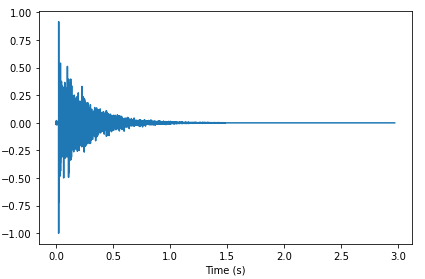
\includegraphics[width=0.75\textwidth]{1_1.png}
			\caption{Импульсный отклик}
			\label{fig:1.1}
		\end{figure}
		
		Теперь построим его спектр
		\begin{lstlisting}[caption=Спектр импульсного отклика]
			transfer = response.make_spectrum()
			transfer.plot()
			decorate(xlabel='Frequency (Hz)', ylabel='Amplitude')
		\end{lstlisting}
		\begin{figure}[H]
			\centering
			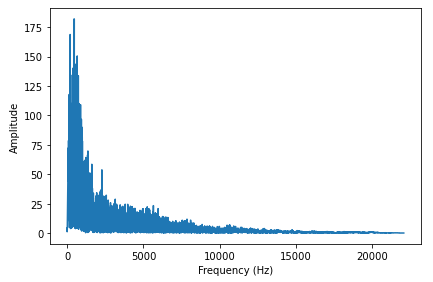
\includegraphics[width=0.75\textwidth]{1_2.png}
			\caption{Спектр импульсного отклика}
			\label{fig:1.2}
		\end{figure}
		
		Теперь возьмем другой сигнал - звук скрипки
		\begin{lstlisting}[caption=Звук скрипки]
			violin = read_wave('res/92002__jcveliz__violin-origional.wav')
			
			start = 0.11
			violin = violin.segment(start=start)
			violin.shift(-start)
			
			violin.truncate(2**16)
			violin.zero_pad(2**17)
			
			violin.normalize()
			violin.plot()
			decorate(xlabel='Time (s)')
		\end{lstlisting}
		\begin{figure}[H]
			\centering
			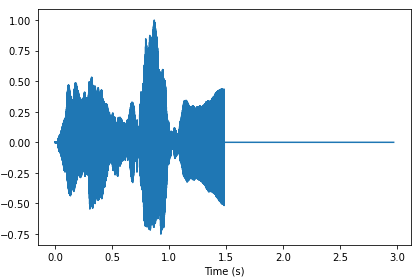
\includegraphics[width=0.75\textwidth]{1_3.png}
			\caption{Спектр импульсного отклика}
			\label{fig:1.3}
		\end{figure}
		
		Построим его спектр, умножим ДПФ сигнала на передаточную функцию и преобразуем обратно в волну
		\begin{lstlisting}[caption=Визуализация сигнала]
			spectrum = violin.make_spectrum()
			
			output = (spectrum * transfer).make_wave()
			output.normalize()
			
			output.plot()
		\end{lstlisting}
		\begin{figure}[H]
			\centering
			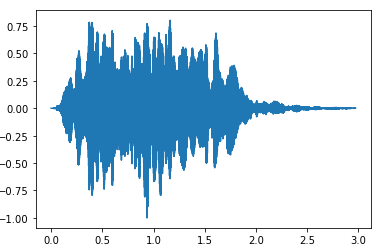
\includegraphics[width=0.75\textwidth]{1_4.png}
			\caption{Визуализация сигнала}
			\label{fig:1.4}
		\end{figure}
		
		Прослушаем
		\begin{lstlisting}[caption=Прослушивание результата]
			output.make_audio()
		\end{lstlisting}
	
		Теперь лишнюю ноту в начале не слышно
		
		Попробуем добиться таких же результатов с использованием \texttt{np.convolve} и \texttt{scipy.signal.fftconvolve}
		
		Для начала, избавимся от нулевого отступа
		\begin{lstlisting}[caption=Избавляемся от нулевого отступа]
			response.truncate(2**16)
			response.plot()
		\end{lstlisting}
		\begin{figure}[H]
			\centering
			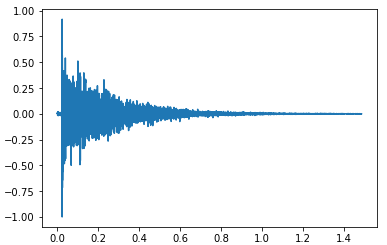
\includegraphics[width=0.75\textwidth]{1_5.png}
			\caption{Избавились от нулевого отступа}
			\label{fig:1.5}
		\end{figure}
		\begin{lstlisting}[caption=Избавляемся от нулевого отступа]
			violin.truncate(2**16)
			violin.plot()
		\end{lstlisting}
		\begin{figure}[H]
			\centering
			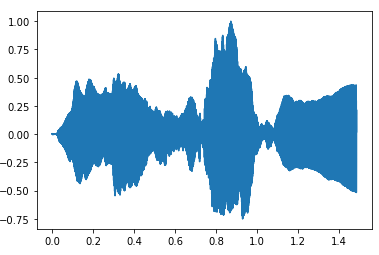
\includegraphics[width=0.75\textwidth]{1_6.png}
			\caption{Избавились от нулевого отступа}
			\label{fig:1.6}
		\end{figure}
		
		Теперь сравним с \texttt{np.convolve}
		\begin{lstlisting}[caption=Cравниваем с \texttt{np.convolve}]
			output2 = violin.convolve(response)
			output2.plot()
			len(output), len(output2)
			
			Output
			(131072, 131071)
		\end{lstlisting}
		\begin{figure}[H]
			\centering
			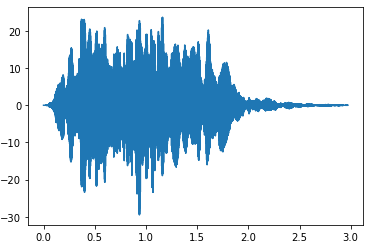
\includegraphics[width=0.75\textwidth]{1_7.png}
			\caption{Cравниваем с \texttt{np.convolve}}
			\label{fig:1.7}
		\end{figure}
		
		Видим, что сигналы похожи, хотя длина одного совсем чуть-чуть отличается от другого.
		
		Теперь поэкспериментируем с \texttt{scipy.signal.fftconvolve}. Этот метод использует БПФ, поэтому он быстрее
		\begin{lstlisting}[caption=Используем \texttt{scipy.signal.fftconvolve}]
			from thinkdsp import Wave
			
			import scipy.signal
			ys = scipy.signal.fftconvolve(violin.ys, response.ys)
			output3 = Wave(ys, framerate=violin.framerate)
			output3.plot()
		\end{lstlisting}
		\begin{figure}[H]
			\centering
			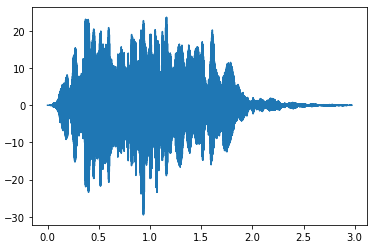
\includegraphics[width=0.75\textwidth]{1_8.png}
			\caption{Используем \texttt{scipy.signal.fftconvolve}}
			\label{fig:1.8}
		\end{figure}
		
		Результат получился такой же, как и в прошлом случае, и звучит также.
		\begin{lstlisting}[caption=Используем \texttt{scipy.signal.fftconvolve}]
			output2.max_diff(output3)
			
			Output
			1.4210854715202004e-14
		\end{lstlisting}
	
		 Разница между \texttt{np.convolve} и \texttt{scipy.signal.fftconvolve} = 1.4210854715202004e-14
		
		
	\end{enumerate}
	\newpage
	
	\section{Упражнение 10.2}
	
	\begin{enumerate}
		
		\item{Задание}
		
		Смоделируйте двумя способами звучание записи в том пространстве, где была измерена импульсная характеристика, как сверткой самой записи с импульсной характеристикой, так и умножением ДПФ записи на вычисленный фильтр, соответсвующий импульсной характеристике.
		
		\item{Ход работы}
		
		В качестве примера я взял звук волныки. Визуализируем его.
		\begin{lstlisting}[caption=Звук волынки]
			response = read_wave('res/bagpipe_music.wav')
			
			start = 0
			duration = 5
			response = response.segment(duration=duration)
			response.shift(-start)
			
			response.normalize()
			response.plot()
			decorate(xlabel='Time (s)')
		\end{lstlisting}
		\begin{figure}[H]
			\centering
			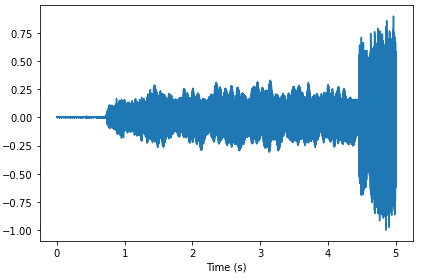
\includegraphics[width=0.75\textwidth]{2_1.png}
			\caption{Звук волынки}
			\label{fig:2.1}
		\end{figure}
		 
		
		Вычислим спектр
		\begin{lstlisting}[caption=Вычисляем спектр]
			transfer = response.make_spectrum()
			transfer.plot()
			decorate(xlabel='Frequency (Hz)', ylabel='Amplitude')
		\end{lstlisting}
		\begin{figure}[H]
			\centering
			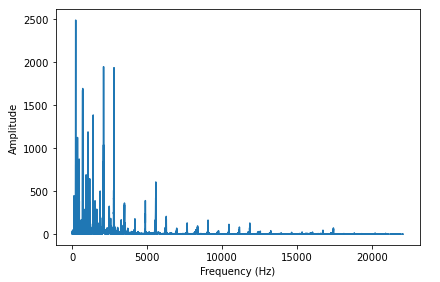
\includegraphics[width=0.75\textwidth]{2_2.png}
			\caption{Спектр звука}
			\label{fig:2.2}
		\end{figure}
		
		Рассмотрим передаточную функцию в логарифмическом масштабе
		\begin{lstlisting}[caption=Передаточная функция в логарифмическом масштабе]
			transfer.plot()
			decorate(xlabel='Frequency (Hz)', ylabel='Amplitude',
			xscale='log', yscale='log')
		\end{lstlisting}
		\begin{figure}[H]
			\centering
			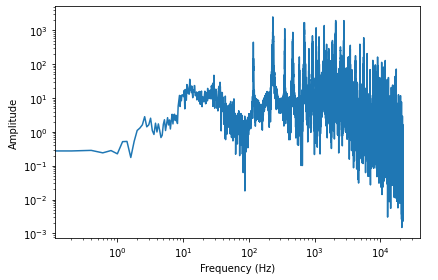
\includegraphics[width=0.75\textwidth]{2_3.png}
			\caption{Передаточная функция в логарифмическом масштабе}
			\label{fig:2.3}
		\end{figure}
		
		Частота звука волныки = 612
		Возьмем еще один звук с примерно такой же частотой -  звук флейты с частотой = 630
		\begin{lstlisting}[caption=Звук флейты]
			wave = read_wave('res/flute_music.wav')
			
			start = 0.0
			wave = wave.segment(start=start)
			wave.shift(-start)
			
			wave.truncate(len(response))
			wave.normalize()
			wave.plot()
			decorate(xlabel='Time (s)')
		\end{lstlisting}
		\begin{figure}[H]
			\centering
			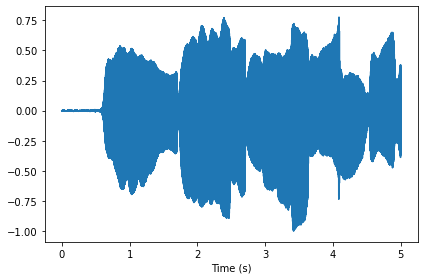
\includegraphics[width=0.75\textwidth]{2_4.png}
			\caption{Звук флейты}
			\label{fig:2.4}
		\end{figure}
		
		Сравним спектры волынки и флейты
		\begin{lstlisting}[caption=Сравниваем спектры]
			len(spectrum.hs), len(transfer.hs)
			
			Output
			(110251, 110251)
			
			spectrum.fs
			Output
			array([0.00000e+00, 2.00000e-01, 4.00000e-01, ..., 2.20496e+04,
			2.20498e+04, 2.20500e+04])
			
			transfer.fs
			Output
			array([0.00000e+00, 2.00000e-01, 4.00000e-01, ..., 2.20496e+04,
			2.20498e+04, 2.20500e+04])
		\end{lstlisting}
	
		Спектры совпадают
		
		Теперь трансформируем запись
		\begin{lstlisting}[caption=Траснформация записи]
			output = (spectrum * transfer).make_wave()
			output.normalize()
		\end{lstlisting}
		
		И сравним оригинал с транформацией
		\begin{lstlisting}[caption=Оригинальный звук]
			wave.plot()
		\end{lstlisting}
		\begin{figure}[H]
			\centering
			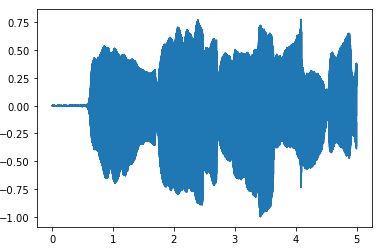
\includegraphics[width=0.75\textwidth]{2_5.png}
			\caption{Оригинальный звук}
			\label{fig:2.5}
		\end{figure}
		\begin{lstlisting}[caption=Трансформированный звук]
			output.plot()
		\end{lstlisting}
		\begin{figure}[H]
			\centering
			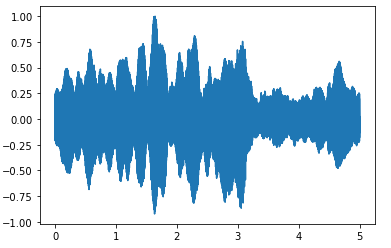
\includegraphics[width=0.75\textwidth]{2_6.png}
			\caption{Трансформированный звук}
			\label{fig:2.6}
		\end{figure}
	
		По звучанию трансформированный звук стал похож на звук из космоса.
		
		Теперь можно сказать, что все эти проделанные операции похожи на свертку. Попробуем применить \texttt{convolve}
		\begin{lstlisting}[caption=Оригинальный звук]
			convolved2 = wave.convolve(response)
			convolved2.normalize()
			convolved2.make_audio()
		\end{lstlisting}
		
		Результат звучит ожидаемо точно также, как и трансформированная запись.
		
	\end{enumerate}
	\newpage
	
	\section{Вывод}
	
	В результате выполнения лабораторной работы получены навыки работы с фильтрами и импульсными характеристиками.

\end{document}